\chapter{Introduction}

This report documents the work done in relation with project in DTU
course 02285 on ``Artificial Intelligence''.  This particular project
explores the use of AI (Artificial Intelligence) in the context of the
Sokoban game.

\section{Background and Rules}

Sokoban (means Warehouskeeper) was created in 1980 by Japanese
software company. The object of the game is to place boxes on goal
squares (their storage location).  Each level consists of a number of
goal squares and a corresponding number of boxes sorrounded by a
wall. This is called the floor plan (or board). To achieve the
objective, the user is represented with as a player able to move in
the directions: up, down, left and right. Boxes can not be pulled,
only pushed. \citep{cgw:sokoban}


Player and boxes can stand on goal squares. If a wall occupies a space
nothing else can be there and the wall cannot be moved from that
space.  The floor plan should be completely enclosed by a continuous
wall.

The game itself is rich in complexity and difficulty can vary from
very easy to incredibly complex, for both human players and automatic
solvers. This of course depends on the initial floor plan.

The high game complexity stems from the many different different
choices available to the player at each game state.

Figure \ref{fig:soko-org-screen} shows the floor plan of the first
level original game.

\begin{figure}
  \centering
  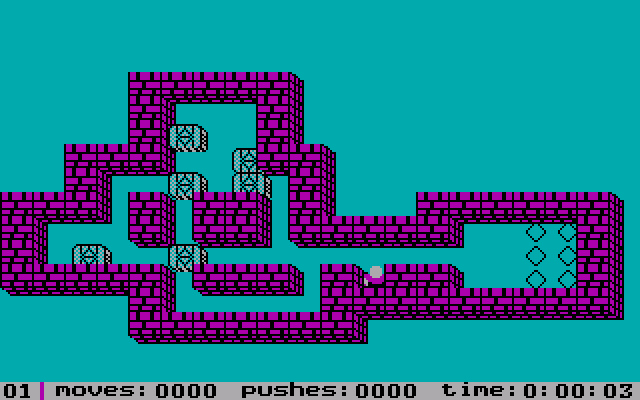
\includegraphics[width=0.7\textwidth]{sokoban-screenshot}
  \caption{Screenshot of the original Sokoban game. From Wikipedia:
    \url{http://en.wikipedia.org/wiki/Sokoban}.}
  \label{fig:soko-org-screen}
\end{figure}
\section{Problem Formulation}



